%%%%%%%%%%%%%%%%%%%%%%%%%%%%%%%%%%%%%%%%%%%%%%%%%%%%%%%%%%%%%%%%%%%%%%%%%%%%%%%%
%
% 2.1.4: Delta-Sigma Stability and Performance Limitiations
%
%%%%%%%%%%%%%%%%%%%%%%%%%%%%%%%%%%%%%%%%%%%%%%%%%%%%%%%%%%%%%%%%%%%%%%%%%%%%%%%%

Ideal linear models are useful for building a conceptual framework and initial system
design and testing. However, practical system designs must account for non-ideal
characteristics and real world limitations. Often the realized performance of a particular
\DSm is vastly different from the ideal theoretical performance. In some cases, failure
to account for realistic limitations may yield a converter which is unstable or fails t
o meet design requirements. Thus, the following sections will address the concepts
of system stability and realizable performance limitations.

\subsubsection{Stability}
A linear time-invariant (LTI) system is said to be stable in the
bounded-input/bounded-output (BIBO) sense if its output is absolutely summable (or
integrable) when stimulated with a summable (or integrable) input signal. System stability
will be defined within this context as follows: A \DSm is said to be stable if for any
bounded input, $x$, and associated error signal, $e$, the system output, $y$, remains
bounded \cite{schreier_empirical_1993}. However, this definition alone is insufficient to
guarantee the realization of a stable system because the output and internal signals are
inherently bounded.

Recall that NTFs and STFs are complex rational functions. Thus, the location of the poles
must be constrained for stability. For discrete functions, the pole locations must be
within the unit circle. Similarly, for continuous functions, the poles must be in the left
half plane. It should also be understood that there exists a non-linear quantizer gain
which is a function of the quantizer input-output relationship. Recall from control
theory that the root locus of a LTI system is defined as the family of curves which
illustrate the locus of the open-loop zeros and poles as function of system gain. Figure
\ref{fig:rlocus} illustrates the root locus for a fourth-order low-pass $\Delta\Sigma$
modulator.
%-------------------
\begin{figure}[htb]
 \centering
 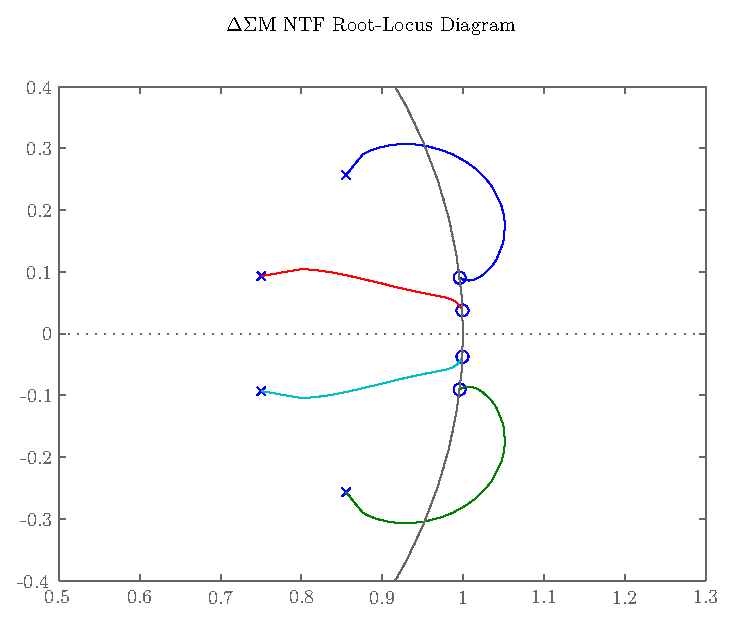
\includegraphics{./final_figures/rlocus.eps}
 \caption{Root-Locus Diagram}
 \label{fig:rlocus}
\end{figure}
%-------------------
Notice in Figure \ref{fig:rlocus} that the poles travel outside the unit circle for
certain values of quantizer gain. This results in system instability and must be avoided
at all costs. However, this phenomenon is the result of signal-dependent non-linear gain
and can only be discovered through exhaustive simulation. This example only serves to
illustrate the reality of unintended system instability as a function of the quantizer
input-output relationship. It should be noted that stability for higher order systems is
very poorly understood and can only be guaranteed through exhaustive simulation.

\subsubsection{Limit Cycles}
It has been shown that when a \DSm is stimulated by a DC input which can be expressed as
a rational number $\alpha/\beta$, when normalized with respect to the quantizer step
$\Delta$, the output is periodic with a period which is a multiple of the denominator
$\alpha$ \cite{friedman_structure_1988}. These oscillations are referred to as limit
cycles and manifest themselves as unexpected spurs in the output spectrum.  Contemporary
designs have idle tone detection and utilize dither to whiten the \DSm output spectrum
\cite{kozak_oversampled_2003}. Limit cycles may also be induced when nonlinear system
dynamics force root oscillation back and forth across the marginal stability threshold
(i.e. the unit circle in Figure \ref{fig:rlocus})\cite{ngai_wong_dc_2003}. Similar to
stability, limit cycles are exceedingly difficult to predict, especially for higher order
systems. As such, exhaustive simulation is critical in the \DSm design cycle.

\subsubsection{Performance Limitations\cite{cherry_continuous-time_1999}}
The hardware implementation of any system design, regardless of application or type, is
always subject to the physical limitations of technology. While \DSms are no different,
they are more sensitive to specific types of nonidealities. 

Discrete-time \DSms are typically realized with switched capacitor circuits and are built
around operational amplifiers (op amps). As such, they are limited by the nonideal op amp
 characteristics. For instance, finite op amp gain results in 'leaky' integrators. This
causes the zeros to move inside the unit circle (off the $j\omega$ axis) resulting in
less noise attenuation within the operational region. Secondly, finite bandwidth effects
manifest themselves as a non-zero settling error. If the error is linear the impact is
largely negligible. However, nonlinear settling errors can only be offset by increasing
the bandwidth of the op amps which can prove difficult for large sampling frequencies.
Finally, finite slew rate, output swing limitations, and gain nonlinearity all degrade the
system fidelity by introducting nonlinear distortion. This distortion is apparent as
harmonics in the output spectrum.

Continuous-time \DSms suffer from excessive loop delay which is defined as the delay
between the sample clock edge and the output transition edge as seen at the feedback
reentry point. This phenomenon causes a significant deviation from the intended frequency
response, directly impacting dynamic system performance if left unaccounted. Similarly, 
sample clock jitter also has a direct impact on system performance by whitening the
in-band noise floor if the OSR rate is not sufficiently high.

A detailed explanation of methods and techniques to offset the myriad of performance
limitations is well beyond the scope of this work. However, it is clear that a generally
robust approach at the outset of system design is essential for realizing \DSms with
ambitious dynamic characteristics.





